\documentclass[12pt]{article}
\usepackage{graphicx}
\begin{document}
\section{Detector Operations }
Problems with the CMS magnet continued through the quarter.  Since March the �Cold Box�(CB) that produces	 Liquid He	for the operation of the CMS magnet	has	shown problems, aftern an incident where compressor oil contaminated the CB circuit. For definitive	recovery, the system	requires an	
overall cleanup	which takes several months. Meanwhile, the CERN cryo group,	in collaboration	
with the CMS Technical Coordination, has	been	
trying to find a way to operate the CB with	a reasonable Duty Cycle ($\ge 70\%$)	that	would	allow	
operation	of	the	magnet	synchronized	with	
physics	operation	of	the	LHC	until	the	Year	end	
technical	stop.  After a number of corrective actions, performance of the magnet has improved and it appears this goal is being met. 
 
 Figure \ref{fig:lumi} shows the total luminosity delivered and recorded by CMS during 2015.  Of this data, approximately 0.40 fb$^{-1}$ is with the magnetic field off or below  nominal value.
\begin {figure}[h]
\begin{center}
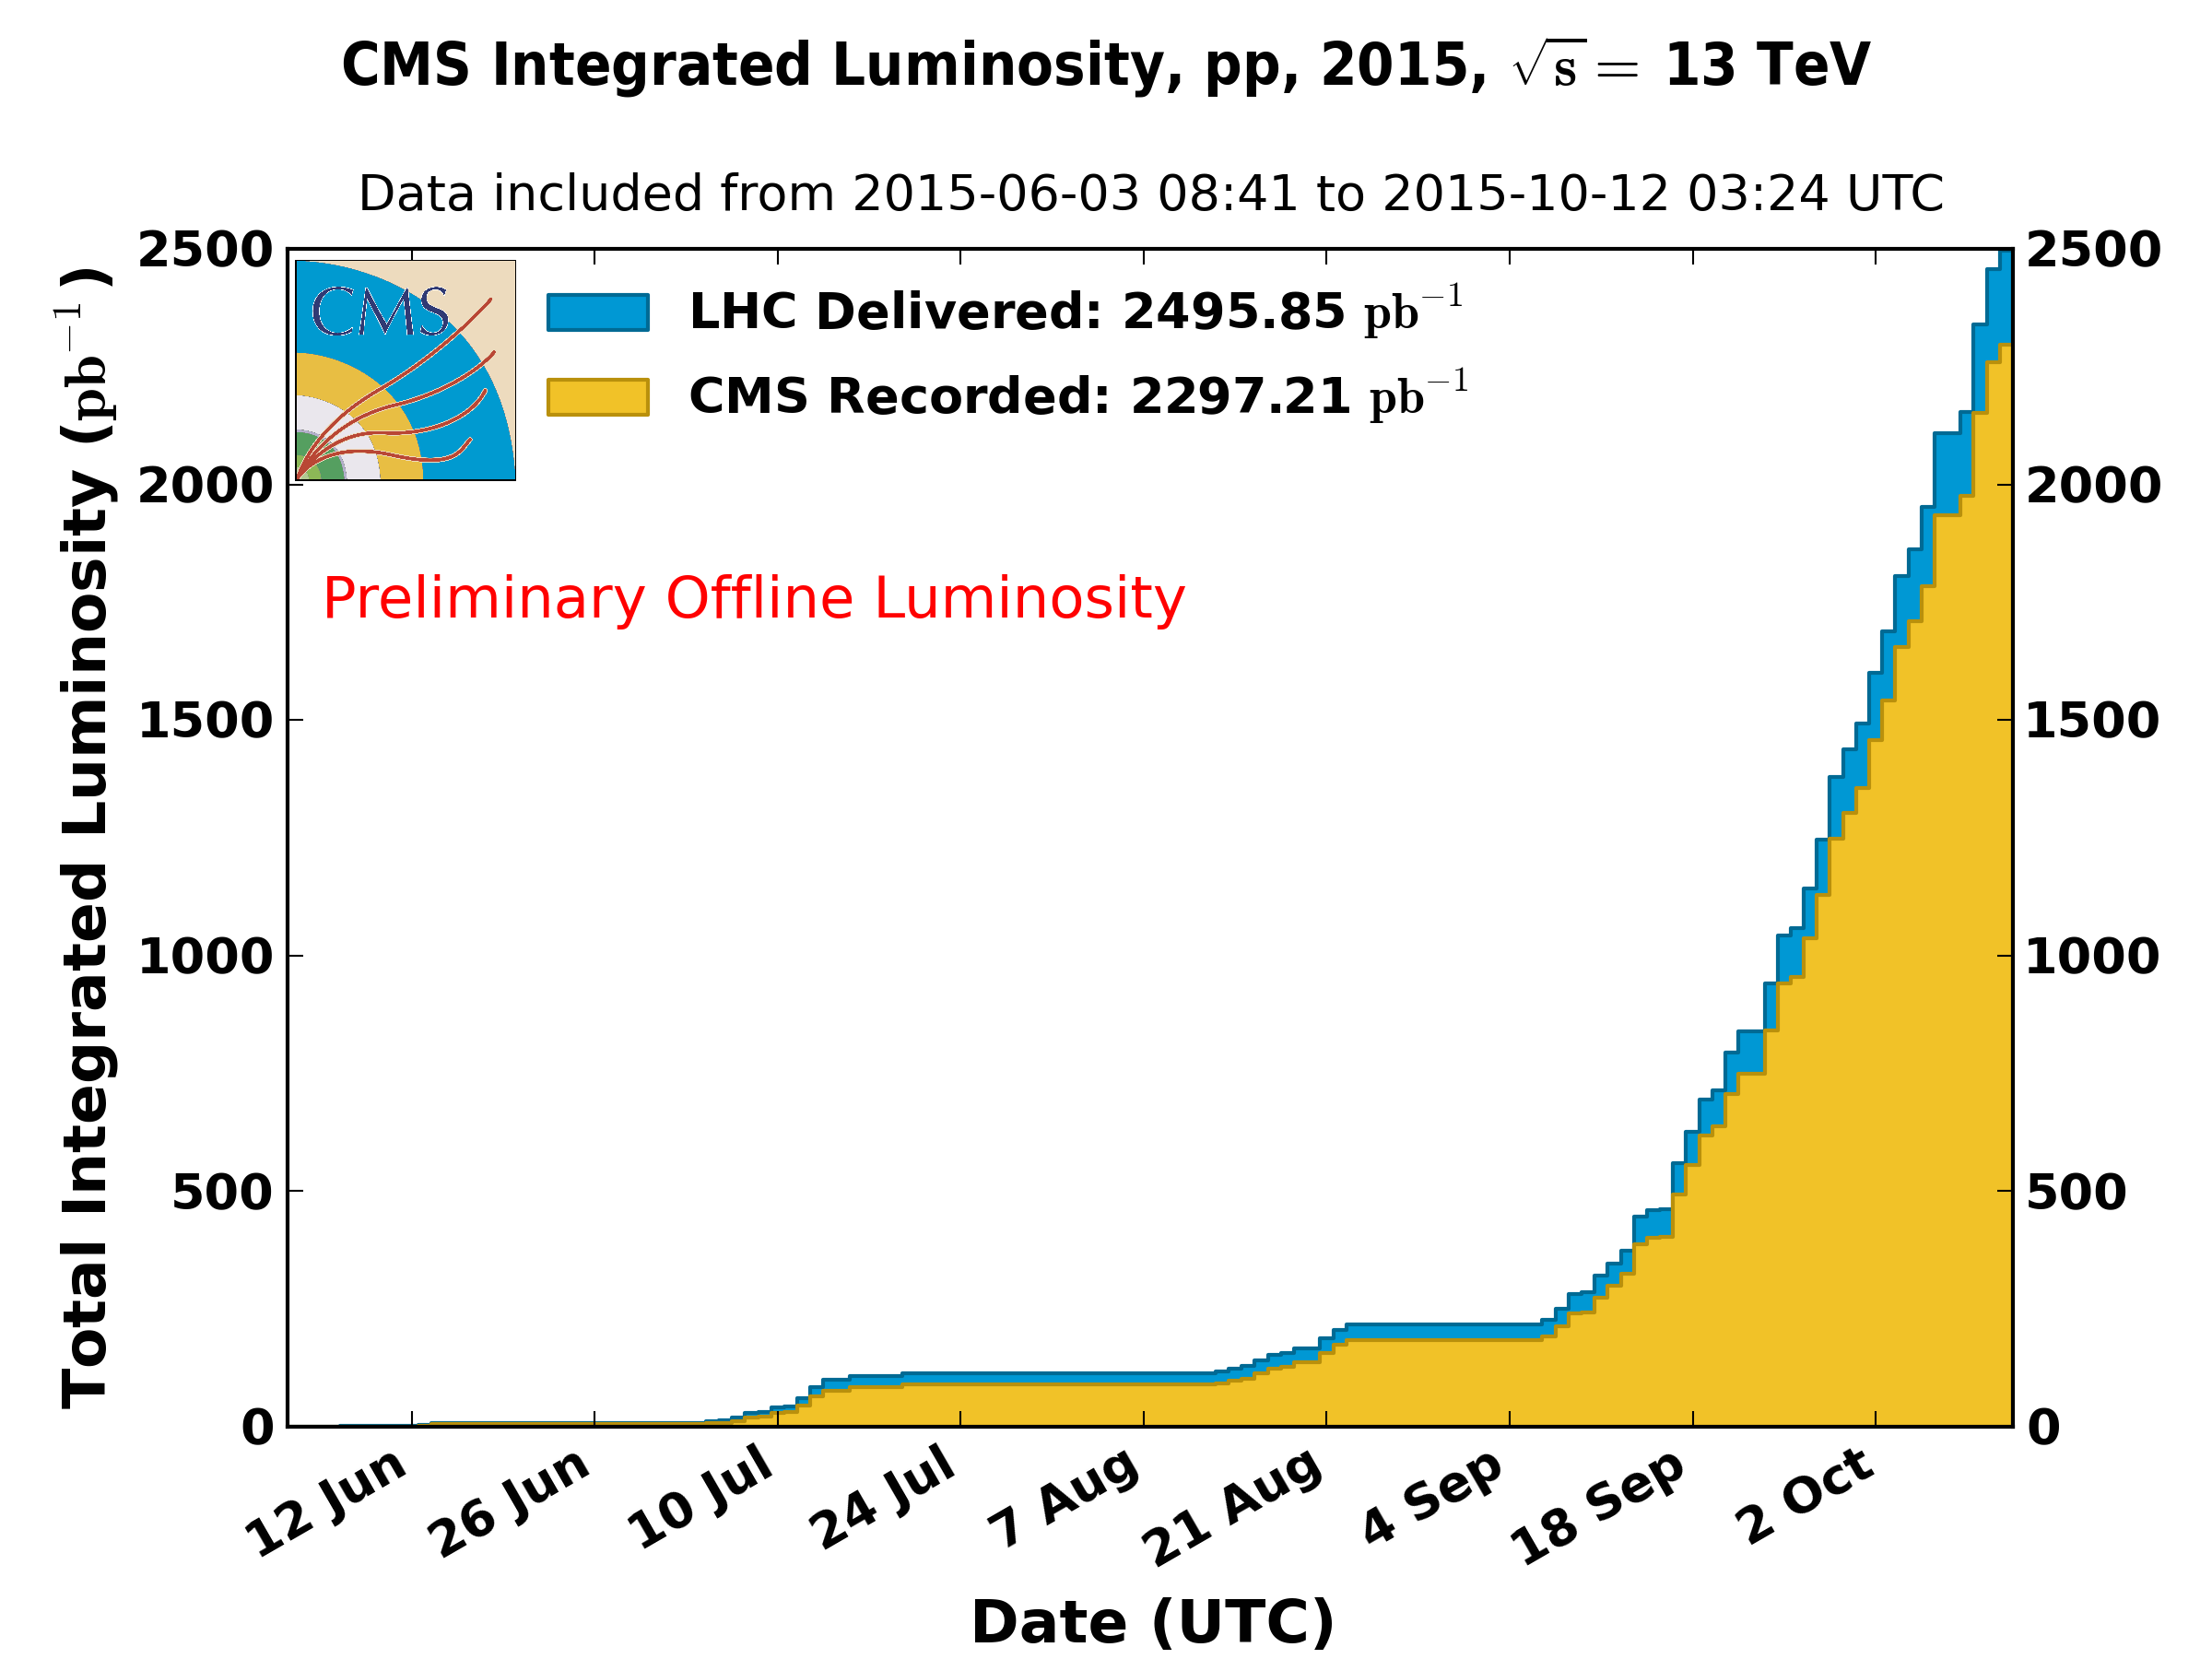
\includegraphics  [width=4in] {int_lumi_per_day_cumulative_pp_2015.png}
\caption{Cumulative offline luminosity versus day delivered to (blue), and recorded by CMS (orange) during stable beams and for p-p collisions at 13 TeV centre-of-mass energy in 2015. The delivered luminosity accounts for the luminosity delivered from the start of stable beams until the LHC requests CMS to turn off the sensitive detectors to allow a beam dump or beam studies. Given is the luminosity as determined from counting rates measured by the luminosity detectors after offline validation. This preliminary calibration is based on short van-der-Meer scans performed routinely by LHC in every fill.}
\label{fig:lumi}
\end{center}
\end{figure}

With this quarterly report we begin to give metric performance results.   These are presented in each sub-detector section below.  

\subsection{BRIL }
The highlight of this quarter was the successful calibration of the PLT and other luminosity
detectors using a full VdM scan. Due to readiness of the detector and the software the PLT
provided the fastest turnaround of all LHC detectors in reporting luminosity to LHC. 
Furthermore, the calibration agrees within 1\% with preliminary calibrations from previous beam 
scans. The CMS detector is in the position to publish the luminosity online with 99\% uptime. 

In addition to the trigger based on 
triple coincidences, PLT has implemented a second trigger to randomly select the bunch crossings 
for saving full particle track information. This trigger mode is in the commissioning phase. It
allows comparative systematic studies and potentially improves the luminosity uncertainty. 

\begin{table}[htdp]
\caption{BRIL Milestones}
\begin{center}
\begin{tabular}{|l|l|r|r|}
\hline
Subsystem&Description&Scheduled&Achieved\\
\hline
BRIL & Hardware installed& Jan & Jan\\
\hline
BRIL& Ready to deliver Lum& March & March \\
\hline
BRIL & Ready to deliver bkg nums& May & May\\
\hline
\end{tabular}
\end{center}
\label{BRILMIlestones}
\end{table}%

\begin{table}[htdp]
\caption{BRIL Metrics}
\begin{center}
\begin{tabular}{|l|r|}
\hline
Metric&Performance\\
\hline
Fraction of telescopes operational & 14/16\\
\hline
Efficiency of delivery of lumi histograms &100\% \\
\hline
Uptime of lumi  histogram production &100\% \\
\hline
\end{tabular}
\end{center}
\label{BRILMetrics}
\end{table}%

\subsection{Tracker }
The tracker system has been performing well and has met its milestones. 
There had been an ongoing problem with condensation in the pneumatic control lines for the cooling
system which  has been traced to short sections of plastic
tubing in the system. The plan is to replace these short sections
with aluminum jacketed pipe in the year end technical stop and
to mitigate the problem with bleed valves in the meantime.


\subsubsection{Strips }

Strips have accounted for 4\% of the lost lumi since the start of the
high intensity running. We continue to try and recover problematic
FEDs (less than 1\% of the Strips), but the emphasis is now on smooth
data taking rather than detailed channel recovery.

\subsubsection{Pixels }

Major downtime from the pixels has come from the testing of Heavy Ion
firmware for the pixel fed. As the request for firmware that could run
at a much higher rate for heavy ion collisions was made in May 2015,
the opportunity to develop with beam in 2012-2013 was lost, and we did not
fully develop an alternative testing method during Long Shutdown 1 (LS1).
The firmware passes all tests outside of collisions, and we are left with
using collisions to fully map out the areas of problems with the heavy
ion firmware. The pixels accounted for 21\% of the lost lumi since the
start of the high intensity running. 98.6\% of the pixel tracker channels
are working. 99.8\% of the FPiX channels are working.




\begin{table}[htdp]
\caption{Tracker Milestones}
\begin{center}
\begin{tabular}{|l|l|r|r|}
\hline
Subsystem&Description&Scheduled&Achieved\\
\hline
Tracker & Installation and checkout& & Achieved\\
\hline
Tracker & Tracker operate -15C & & Achieved\\
\hline
Tracker & Pixel operate -10C & & Achieved\\
\hline
Tracker& Ready for proton beams& March & March\\
\hline
\end{tabular}
\end{center}
\label{TrackerMilestones}
\end{table}%

\begin{table}[htdp]
\caption{Tracker Metrics}
\begin{center}
\begin{tabular}{|l|c|c|}
\hline
 &Pixels&Strips\\
\hline
\% Working channels & 98.6 & 97.5 \\
\hline
Fraction of deadtime attributed& 21\%& 4\%\\
\hline
\end{tabular}
\end{center}
\label{TrackerMetrics}
\end{table}%


\subsection{ECAL }
All parts of ECAL (EB/EE/ES) are taking data normally.   Substantial effort has been devoted to improving the data-taking efficiency of ECAL by simulating higher than normal data acquisition rates and solving the rare errors that occurred. The ECAL optical links to the legacy and upgraded calorimeter triggers have been successfully validated and the detector has been synchronized with the rest of CMS using beam splash events and proton-proton collisions data.  

In addition, the laser used for calibrating the crystals has been operating well.  At the end of Run 1 there was a laser power stability issue that was traced to a flawed humidity sensor, which has since been replaced.  With that replacement the operation has been stable with no power loss in the system.

A successful test beam campaign was conducted in Sep  2015 using electrons provided by the H4 beamline at the CERN-SPS. Measurements of highly irradiated PbWO4 crystals were recorded, with special two-sided readout, to study the changes in light collection efficiency as a function of the radiation-induced crystal transparency change.

\begin{table}[htdp]
\caption{ECAL Milestones}
\begin{center}
\begin{tabular}{|l|l|r|r|}
\hline
Subsystem&Description&Scheduled&Achieved\\
\hline
ECAL & Finish HV Install& Feb & May\\
\hline
ECAL & Baseline levels zero suppression& March & March \\
\hline
ECAL & Complete install HV calib system & April &May\\
\hline
ECAL & Selective readout& June & First pass completed\\
\hline
ECAL & Trigger thresholds & June &First pass completed\\
\hline
ECAL & Zero suppression thresholds & June & First pass completed \\
\hline
\end{tabular}
\end{center}
\label{ECALMilestones}
\end{table}%

\begin{table}[htdp]
\caption{ECAL Metrics}
\begin{center}
\begin{tabular}{|l|r|}
\hline
Metric&Performance\\
\hline
Fraction of channels operational: EB& 99.1\%\\
\hline
Fraction of channels operational: EE& 98.9\% \\
\hline
Fraction of channels operational: ES& 98.4\% \\
\hline
Fraction of deadtime attributed& 14\%\\
\hline
Resolution performance & TBD\\
\hline
\end{tabular}
\end{center}
\label{ECALMetrics}
\end{table}%





\subsection{HCAL}
In this quarter, the HCAL project has focused on two tasks:  
the operation of the HCAL detector for LHC collisions at 13 TeV in Run II, 
and the development and installation of the Phase I upgrades.

With Run II underway, a major emphasis has been the collection of high quality data from all HCAL subsystems (HBHE, HF, and HO). To accommodate collisions with 25 ns bunch spacing, new local reconstruction code has been developed and commissioned; the improved algorithm has substantially improved the mitigation of out-of-time pileup. Using data taken early in Run II, the calibration of the HBHE and HF sub-detectors has been adjusted, and corresponding corrections to the Level-1 trigger look-up tables have been implemented.

The long-term stability of the response of HCAL photo-detectors in Run II is being monitored using the LED calibration system. The average gain of the legacy HBHE hybrid photodiodes (HPDs) has been nearly stable over the last six months at the level of 1\%\ , although a slow drift, either up or down, of the individual HPD gains with time is observed, comparable to effects seen in Run I. The gains of the new PMTs for the HF are stable within 1\%\, 
with no evidence of gain loss as a function of integrated luminosity. 
Similarly, the gain of the HO Silicon PhotoMultipliers (SiPMs) is very stable, with no sign of dependence on the magnetic field.
\begin{table}[htdp]
\caption{HCAL Milestones}
\begin{center}
\begin{tabular}{|l|l|r|r|}
\hline
Subsystem&Description&Scheduled&Achieved\\
\hline
HCAL& Fully functional HCAL in CRAFT runs & March & March\\
\hline
HCAL& prepared to do HF Phase scan & &\\
&and $\phi$ symmetry calibration analysis& May& May\\
\hline
HCAL&New HBHE backend operating in& &\\
& parallel with legacy system& July & July\\
\hline
\end{tabular}
\end{center}
\label{HCALMilestones}
\end{table}%

The status of the HCAL metrics is as follows:
\begin{itemize}

\item Fraction of channels working\\
in HF, 1 channel out of 1728 dead \\
in HBHE, 7 channels out of 5184 dead\\
in HO all 2150 channels work.\\
In total $>$ 99.9\%\ working channels
\item Fraction of downtime attributable to HCAL since LS2, 0.5\% \\ 
2.7pb-1 lost of 562 pb-1
\item Intercalibration uniformity between individual HCAL towers\\
HB:� depth 1:� 3-4\%  \\
HE: depth 1:  $\approx$1-2\%  \\
HE:�depth 2,3: 3-4\% \\
HF: depth 1: 1-1.5\%  depth 2: ~3\% (still some outliers)\\
\end{itemize}

Unfortunately, there have been issues that led to a significant loss of data during data certification.
There were issues with the loss of synchronization between the HF backends and fronts ends
that cost 75~pb$^{-1}$ of bad data and an issue with a low voltage power supply for HF that cost 
10~pb$^{-1}$ of bad data. These issues have been resolved. There is also an issue with 
$\mu$HTR registers being occasionally  corrupted when a detector re-configuration is issued.
This problem is still under study, but a temporary work-around has been implemented.


\subsection{EMU }
The transition to 25 ns LHC beam bunch spacing went smoothly
for the CSC system. Figure \ref{fig:emu} shows  the track segment
times in the CSC readout window displaying the 25 ns beam structure
clearly.
\begin {figure}[h]
\begin{center}
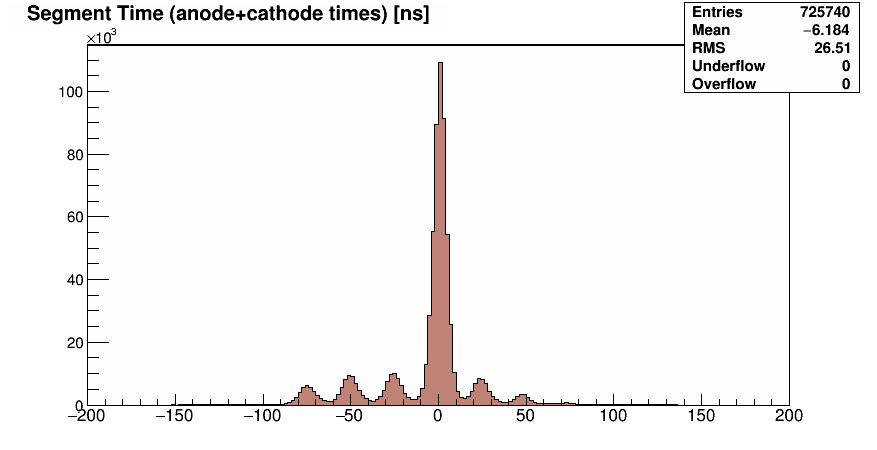
\includegraphics  [width=4.5in] {mu_seg_time_25ns_psm.png}
\caption{The timing of CSC Segments relative to the triggered
beam crossing in 25 ns collision data.}
\label{fig:emu}
\end{center}
\end{figure}

The spatial resolution for reconstructed hits on CSC chambers
was measured from collision data. The resolution varies by
chamber type, with a median value of 128 $\mu$m. The resolutions
are very close to the values from Run 1, aside from the ME1/1
chambers, where the resolution on the inner region (ME1/1a) has
gone from 64 $\mu$m to 51 $\mu$m. This improvement is largely due to
the removal of the 3-to-1 cathode strip ganging in this region
performed during the LS1.

A sample of $Z\rightarrow\mu\mu$ events from Run 2 collision data were used to make
the first measurement of the efficiencies for CSC segments and
trigger primitives (LCT). The average for all 540 chambers is
greater than 96\% with a few outliers from known outstanding
chamber issues and low statistical accuracy. The efficiencies
are more uniform than in Run 1 due to the high fraction of
operational system channels.


 \begin{table}[htdp]
\caption{EMU Milestones}
\begin{center}
\begin{tabular}{|l|l|r|r|}
\hline
Subsystem&Description&Scheduled&Achieved\\
EMU& CSC ready for collisions& May & April \\
\hline
EMU& Calibration for HLT and & &\\
& Offline included in DB & July & delayed\\
\hline
EMU & Fine timing adjustments & & \\
&with collision data completed & July &July \\
\hline
\end{tabular}
\end{center}
\label{EMUMilestones}
\end{table}%

The milestone ``Calibration for HLT and Offline included in DB'' has been delayed.  It is now expected that it will be completed in December. There are technical problems with taking calibration data at Point 5. These have been worked on since July, but they can only be done when CMS is not taking
data. Operational issues that affect physics running are given higher priority. We are using a set of calibration constants from Run 1, except for ME1/1 and
ME4/2 chambers where these constants are not available. For these, we use
typical values for each chamber.  The impact of this delay is low, the reconstruction is quite insensitive 
to the calibration.  The main motivations for the calibration are to represent the cross talk
correctly in the simulation and to allow more precise tracking of gas gain.

\begin{table}[htdp]
\caption{CSC Metrics}
\begin{center}
\begin{tabular}{|l|c|}
\hline
 \% Working channels & 99.3\%  \\
\hline
Fraction of deadtime attributed& 8\%\\
\hline
Median spatial resolution & 128 $\mu$m\\
\hline
\end{tabular}
\end{center}
\label{TrackerMetrics}
\end{table}%

\subsection{DAQ}

DAQ met all its milestones and performing with negligible down time during physics data taking. LHC has not completed the Luminosity ramp up and presently CMS is taking data with 80 kHz Level 1 trigger rate and average event size of 650 kB which is below the design throughput of the DAQ2. 

Event Building performance demonstrated in emulation runs that it could sustain event building at 100 kHz L1 accept rate with a margin of 1.5 times the run 1 event size of 750kB. (DAQ I design performance was 100 kHz L1 accept rate for 1 MB Events) with full DAQ chain - event building, High Level Trigger  (HLT) processing (actually emulated as sleep) and collecting HLT selected event in to single files per stream ready to be send to tier 0. Actual demonstration, of course, will be with real detector data with full HLT menu but for that we need to wait LHC luminosity to increase. 

\begin{table}[h]
\caption{DAQ Milestones}
\begin{center}
\begin{tabular}{|l|l|r|r|}
\hline
Subsystem&Description&Scheduled&Achieved\\
\hline
DAQ& Hardware Installation of DAQ2& & \\
& with new HLT nodes complete& April & April \\
\hline
DAQ& Complete DAQ2 is operational && \\
&for collisions& July &   May\\
\hline
DAQ&$\mu$TCA DAQ link commissioned & & \\
&for new trigger and HCAL FEDs& July &  June \\
\hline
DAQ&DAQ2 with Run I design performance & Sept. &Sept. \\
\hline
\end{tabular}
\end{center}
\label{DAQMilestones}
\end{table}%

\begin{table}[htdp]
\caption{DAQ Metrics}
\begin{center}
\begin{tabular}{|l|c|}
\hline
 Dead time due to trigger throttling& 0.007\%  \\
\hline
Downtime due to DAQ& negligible\\
\hline
Median spatial resolution & 128 $\mu$m\\
\hline
\end{tabular}
\end{center}
\label{DAQMetrics}
\end{table}%


\subsection{Trigger}
During this quarter the US groups continued their work on the regional calorimeter (RCT) and the endcap muon triggers.  
\subsubsection{Regional Calorimeter Trigger}
During the last three months, the CMS RCT has participated in the 25 ns LHC proton-proton collisions. CMS has switched from calorimeter triggers with the RCT and GCT to triggers with the the RCT and Stage-1 MP7.  Accordingly, the configuration and hardware monitoring were added to the Trigger Supervisor, and the histograms in the online Data Quality Monitoring (DQM) were updated to use the readout from the MP7.  Previously it was reported that the RCT output could be readout via CDAQ using the CTP7. Using this data, a second set of online DQM (emulator and occupancy) histograms were added to the Online DQM of the RCT.


The new HF uHTR links to RCT have been commissioned.  There were still some issues with links going into error and with the HF link synchronization.  This caused effects in the Jet rates which were similar to the ECAL issues. It was mitigated in the same way, using the same firmware as for the ECAL oRMS, but will need further dedicated study outside of physics running.  

\subsubsection{Endcap Muon Trigger}
The Rice University, Northeastern, and University of Florida groups have maintained on-call coverage of the CSC Track-Finder during the reporting period, with only a few instances needing intervention. We eventually had to replace a QPLL module on one sector processor that had occasionally lost synchronization during operations.

The CSC Track-Finder group also participates in the CMS TimeX group, which is part of Run Operations. In that context, the CSC Track-Finder delay buffer depths are being monitored to flag any shifts in the TCDS clock timing, which has been observed by several CMS subsystems. Moreover, we have participated in system tests of the new reset procedure in order to avoid these TCDS timing shifts. 

\begin{table}[h]
\caption{Trigger Milestones }
\begin{center}
\begin{tabular}{|l|l|r|r|}
\hline
Subsystem&Description&Scheduled&Achieved\\
\hline
TRIG&Legacy RCT ready for physics&June &June\\
\hline
TRIG&MPC ready for physics&June &June\\
\hline
TRIG&CSCTF Ready for physics&June & June\\
\hline
TRIG& Stage-1 Layer-1 calorimeter trigger&&\\
& ready for physics &Sept.& Sept.\\
\hline
\end{tabular}
\end{center}
\label{TriggerMilestones}
\end{table}%

\begin{table}[htdp]
\caption{Trigger Metrics}
\begin{center}
\begin{tabular}{|l|c|}
\hline
 Frac legacy RCT channels & 100\%  \\
\hline
Frac of deadtime attributed legacy RCT& 0.18\%\\
\hline
Frac of MPC Channels& 100\%\\
\hline
Frac of EMUTF Channels& 100\%\\
\hline
Frac of deadtime attributed to legacy EMUTF& 0.13\%\\
\hline
Frac of Stage-1 Layer-1 Channels & 100\%\\
\hline
Frac of deadtime attributed to Stage 1 Layer 1 & 0\%\\
\hline
\end{tabular}
\end{center}
\label{TriggerMetrics}
\end{table}%


\end{document}

